% WACV 2026 submission — Clinical Concept Routing
% NOTE: working draft still typeset in single-column LNCS. Target format is the
% WACV/CVPR two-column template (cvpr.sty + ieeenat_fullname.bst); conversion and the
% trim to WACV's 8-page limit are pending (see post-eval task list).
\documentclass[runningheads]{llncs}

\usepackage{graphicx}
\usepackage{amsmath,amssymb}
\usepackage{booktabs}
\usepackage{multirow}
\usepackage{pifont}   % \ding{55} (cross) in the capability columns of tab:compare
\usepackage{xcolor}
\usepackage{tikz}
\usetikzlibrary{arrows.meta,positioning,fit,backgrounds}
\usepackage[hidelinks]{hyperref}

\DeclareMathOperator*{\argmax}{arg\,max}
\newcommand{\todo}[1]{\textcolor{red}{[#1]}}
\newcommand{\casfg}{\mathrm{CAS}_{\mathrm{fg}}}
\newcommand{\Rb}{\mathbb{R}}

\begin{document}

\title{The Route Is the Reason: Clinical Concept Routing\\ for Faithful 3D Medical Segmentation}
\titlerunning{Clinical Concept Routing}

\author{Anonymous WACV 2026 submission}
\authorrunning{Anonymous WACV 2026 submission}
\institute{Paper ID \todo{XXXX}}

\maketitle

\begin{abstract}
Deep segmentation models now rival expert accuracy on brain-tumor benchmarks, yet
clinical adoption lags because their decisions cannot be \emph{faithfully} explained.
The dominant remedy---post-hoc attribution (Grad-CAM, gradients, integrated gradients,
occlusion)---computes a saliency map \emph{after} the prediction; even when such a map scores
well on input-sensitivity tests, it reports \emph{where} the model is sensitive, not \emph{which
clinical concept} a region is, and it is reconstructed from the output rather than read from the
decision. We propose \textbf{Clinical Concept Routing (CCR)}, a different
principle: replace the encoder bottleneck with a routing layer that assigns every image
token to one of $K$ clinically-labeled expert networks. The routing probability
distribution is, simultaneously, the model's clinical concept assignment, the
segmentation mechanism, and a per-voxel explanation---computed in a single forward pass,
with no post-hoc step. CCR is a drop-in bottleneck module; we instantiate it as \textbf{CCR-Net}
(a Swin encoder with a routing bottleneck and a UNETR decoder), detail its router, expert bank, dispatch
mechanism, five-term objective, and three-phase curriculum, and characterize the sense in which its
explanation is structurally faithful, with alignment quality measured by the Concept Alignment
Score (CAS). We argue that a clinical explanation must satisfy two requirements at once: it must be
\emph{concept-labeled}, and it must be \emph{distinct from and causally upstream of} the prediction.
On the BraTS 2024 glioma benchmark these requirements separate three families. Post-hoc saliency
(Grad-CAM, gradients, integrated gradients, occlusion) is upstream but cannot discriminate the
clinical concepts (AUROC $0.52$--$0.73$). The model's own segmentation posterior discriminates them
almost perfectly ($0.98$) but \emph{is} the prediction---it restates the output rather than exposing
what produced it, and its decoder divergence is zero by construction. CCR routing satisfies both:
it discriminates concepts at $0.88$, far above every post-hoc method, while remaining upstream
(DD${>}0$) and intrinsic. We report the full battery openly, including where CCR loses: integrated
gradients and occlusion win deletion \emph{sensitivity}, which they optimize directly, and the
posterior wins discriminability. Two controls show the remaining gap is largely structural rather
than informational---matching the posterior to the router's $16^3$ decision budget removes about
half of it, and on edema the two become statistically indistinguishable---while CCR \emph{exceeds}
the posterior on insertion. Ablations confirm concept alignment is \emph{learned} (it collapses
without the alignment loss) and that warm-up is a stabilizing default, not a requirement. Dropped
\emph{unchanged} into a SegResNet CNN (CCR-SegResNet), the same module reproduces every result from
scratch ($\casfg$ up to $0.96$), so the principle is backbone-agnostic.
\keywords{Interpretability \and Faithfulness \and Medical image segmentation \and
Mixture-of-experts \and Brain tumor}
\end{abstract}

% ====================================================================
\section{Introduction}
% ====================================================================
Brain-tumor segmentation models now match or exceed expert radiologists on benchmark
data, but clinical deployment has not followed. The barrier is not accuracy; it is the
absence of a \emph{trustworthy, verifiable} account of what the model computed and why. A
radiologist asked to act on a segmentation needs to know which clinical concept the model
assigned to each region and to trust that this account reflects the actual computation.

The dominant response is post-hoc attribution: after the model predicts, apply
Grad-CAM~\cite{selvaraju2017gradcam}, integrated gradients~\cite{sundararajan2017ig},
SHAP~\cite{lundberg2017shap}, or attention rollout~\cite{abnar2020rollout} to reconstruct
a saliency map that \emph{approximates} the decision mechanism. The structural problem is
that these methods were designed for single-scalar-output models; in dense prediction
every voxel has its own output, and the extension proceeds through heuristics---averaging
gradients, summing attention weights, approximating Shapley values over spatial
regions---each introducing a gap between the attribution and the actual computation. More
fundamentally, the explanation is built from \emph{byproducts} of computation (gradients,
attention weights), not from the computation itself, and it is a scalar \emph{sensitivity} map,
not a concept assignment. A strong sensitivity method can even score well on input-sensitivity
tests such as the deletion/insertion game~\cite{petsiuk2018rise}---efficiently ranking the
high-leverage voxels---but a high sensitivity score does not make a map a clinical explanation:
it still cannot say \emph{which} concept a region is, and it is reconstructed from the output
rather than being the decision. The right response is to make the decision itself
interpretable~\cite{rudin2019stop}.

We propose a different principle. \textbf{Clinical Concept Routing (CCR)}: in an
encoder--decoder segmentation model, replace the bottleneck with a routing layer that
assigns each image token to one of $K$ clinically-labeled expert networks
\{Background, Necrotic core, Edema, Enhancing tumor\}. The routing distribution, computed
at the bottleneck, is the model's clinical concept assignment for each token, and it
\emph{actively conditions} all downstream computation: it is causally upstream of the
prediction, not derived from it. The explanation is not reconstructed from the
prediction---it \emph{is} the decision mechanism. Because the routing assignment is read
directly from the forward pass, the per-voxel, concept-labeled explanation comes for free,
deterministically, every time the model predicts (Fig.~\ref{fig:arch}).

\paragraph{What a clinical explanation has to be.}
Stating the requirement precisely is what makes the comparison meaningful, so we adopt two
criteria. An explanation must be \textbf{(i) concept-labeled}---it must say \emph{which} clinical
concept a region is, not merely that the region matters---and \textbf{(ii) distinct from and
causally upstream of the prediction}, so that reading it tells us something about how the output
was produced rather than restating the output. These criteria are not rhetorical: each eliminates
a different family. Post-hoc saliency satisfies (ii) but fails (i)---a sensitivity map has no
concept semantics, and empirically the strongest post-hoc method separates the BraTS concepts at
AUROC $0.73$ while integrated gradients and Grad-CAM sit near chance. The model's own segmentation
posterior satisfies (i) trivially and fails (ii) completely: it discriminates concepts at $0.98$
\emph{because it is the concept prediction}, offering no account of what produced it. This is not a
straw baseline---it is free from the same forward pass, and any evaluation of concept explanations
that omits it is incomplete---but an explanation that is identical to the thing being explained is
vacuous. CCR routing is, to our knowledge, the first construction for 3D dense prediction that
satisfies both criteria simultaneously.

\noindent\textbf{Contributions.}
\begin{enumerate}
\item \textbf{The CCR principle and a backbone-agnostic module.} The first method to route
tokens to \emph{clinically labeled} experts at the segmentation bottleneck so that routing is at
once the prediction and a per-voxel, concept-labeled explanation, for 3D dense prediction. CCR
is a drop-in bottleneck module: we instantiate it, \emph{unchanged}, on a Swin transformer
(CCR-Net) and a SegResNet CNN (CCR-SegResNet), and it transfers (Sec.~\ref{sec:method},
Sec.~\ref{sec:backbone}). We detail the router, expert bank, soft/hard dispatch, five-term
objective, and curriculum.
\item \textbf{A faithfulness framework.} We define the Concept Alignment Score (CAS) and Decoder
Divergence (DD), and distinguish faithfulness (structural) from alignment quality (CAS) from
causal relevance (deletion AUC)---three things routinely conflated in the literature
(Sec.~\ref{sec:theory}).
\item \textbf{An honest characterization against \emph{both} competing families.} Under one
identical protocol on all $168$ test cases, we evaluate CCR against four post-hoc baselines
\emph{and} against the segmentation posterior---the intrinsic baseline that concept-explanation
evaluations typically omit. CCR is the only method satisfying both criteria above; we report
plainly that it is not first on any single metric, and we run two controls (a granularity-matched
posterior, and insertion) that isolate how much of the residual gap is decision budget rather than
information (Sec.~\ref{sec:experiments}).
\item \textbf{Ablations} isolating the role of the alignment loss (concept alignment is
learned, not incidental) and of curriculum warm-up (the routing aligns even without it---a
robustness result).
\end{enumerate}

% ====================================================================
\section{Related Work}
% ====================================================================
\subsubsection{Post-hoc attribution.}
Grad-CAM~\cite{selvaraju2017gradcam} weights feature maps by the gradient of the output
w.r.t.\ that feature; integrated gradients~\cite{sundararajan2017ig} integrate gradients
along a baseline path with axiomatic guarantees but no faithfulness guarantee for dense
prediction; SHAP~\cite{lundberg2017shap} approximates Shapley values, intractable in high
dimension; attention rollout~\cite{abnar2020rollout} propagates attention through layers
but conflates attention magnitude with causal contribution. All operate \emph{after}
prediction and produce an input-\emph{sensitivity} map, not a concept assignment. On dense
prediction, strong sensitivity methods (integrated gradients, occlusion) can even score well on
deletion/insertion~\cite{petsiuk2018rise}, yet---as we show (Sec.~\ref{sec:faith})---their maps
do not discriminate the clinical concepts. CCR does not improve post-hoc attribution; it removes
the structural reason it cannot be a concept explanation, by making the decision
intrinsic~\cite{rudin2019stop}.

\subsubsection{Intrinsic interpretability.}
Concept Bottleneck Models~\cite{koh2020cbm} route predictions through a human-readable
concept layer whose activation \emph{is} the explanation; ProtoPNet~\cite{chen2019protopnet}
classifies by prototype similarity (``this looks like that''). Both are designed for
scalar-output classification, neither handles dense prediction, and neither offers a formal
faithfulness statement. CCR extends the intrinsic-interpretability principle to 3D
volumetric segmentation, where the explanation must be per-voxel and concept-labeled.

\subsubsection{Mixture-of-experts routing.}
Sparse MoE~\cite{shazeer2017moe,fedus2022switch,riquelme2021vmoe} was introduced for
\emph{efficiency}: conditional computation that processes each input with a subset of
parameters. Vision and medical adaptations reuse routing for efficiency, domain adaptation,
or missing-modality robustness. None of these works label experts with clinical concepts,
enforce routing--concept alignment with an explicit loss, or treat the routing decision as
the model's explanation. CCR's objective---faithful intrinsic explanation---is different in
kind and requires a different design: clinically-labeled experts, an alignment loss, and
bottleneck placement.

% ====================================================================
\section{Method}\label{sec:method}
% ====================================================================
\subsection{Overview and the CCR principle}
Let an encoder map a multi-modal volume $x\in\Rb^{C_{\text{in}}\times H\times W\times D}$
to a set of bottleneck tokens $\{h_t\}_{t=1}^{N}$, $h_t\in\Rb^{d}$, arranged on a coarse
spatial grid. The CCR module replaces the plain bottleneck with three components: a
\emph{router} that produces, per token, a distribution over $K$ clinically-labeled
experts; an \emph{expert bank} $\{E_k\}_{k=1}^K$; and a \emph{dispatcher} that combines
expert outputs according to the routing. The routing volume $\{p_k(t)\}$ is, at once, (i)
the model's clinical concept assignment, (ii) a quantity that conditions every downstream
computation, and (iii) the explanation read out for the user. We instantiate $K{=}4$ to
match the BraTS annotation protocol exactly: \{Background, NCR, Edema, ET\}.

\paragraph{What kind of explanation this is.}
CCR does not attach a post-hoc saliency map to a fixed black box; it makes the model's
decision interpretable \emph{by construction}~\cite{rudin2019stop}. Because the architecture
must route each region to exactly one clinically-labeled expert \emph{before} the decoder can
act, the routing is a load-bearing, concept-level decision variable---which expert processed a
region, and with what confidence (entropy)---not a heatmap reconstructed from the output. It is
causally upstream of the prediction and, as we measure (DD, Sec.~\ref{sec:theory}), \emph{not}
identical to it; the per-concept experts make it modular, so one can inspect which expert fired
and intervene by ablating it (the deletion analysis of Sec.~\ref{sec:faith}). This is a
different object from a monolithic segmentation posterior and from a post-hoc attribution: the
explanation \emph{is} the decision, read from the computation---so ``is routing just the
prediction?'' misreads the claim. Routing is the concept-level decision that \emph{produces}
the prediction, exposed faithfully rather than reconstructed.

\begin{figure}[t]
\centering
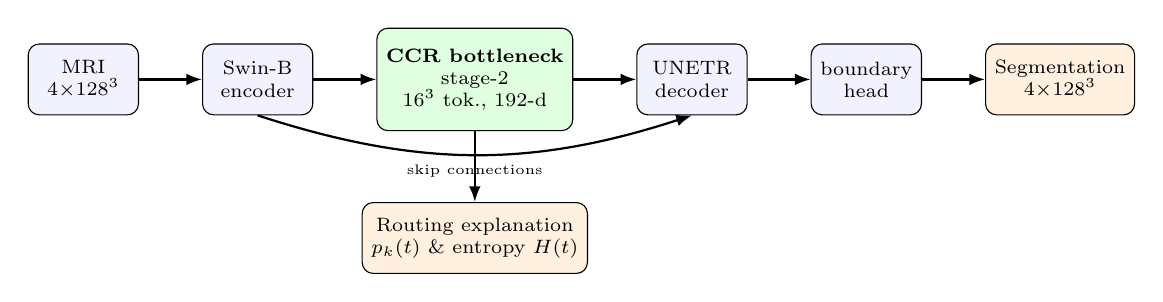
\begin{tikzpicture}[
  node distance=5mm and 8mm,
  box/.style={draw, rounded corners, align=center, minimum height=9mm,
              minimum width=14mm, font=\scriptsize, fill=blue!5},
  ccr/.style={draw, rounded corners, align=center, minimum height=13mm,
              minimum width=20mm, font=\scriptsize, fill=green!12},
  outb/.style={draw, rounded corners, align=center, minimum height=9mm,
              minimum width=16mm, font=\scriptsize, fill=orange!12},
  ar/.style={-{Latex[length=2mm]}, thick}]
\node[box] (mri) {MRI\\$4{\times}128^3$};
\node[box, right=of mri] (enc) {Swin-B\\encoder};
\node[ccr, right=of enc] (ccr) {\textbf{CCR bottleneck}\\stage-2\\$16^3$ tok., $192$-d};
\node[box, right=of ccr] (dec) {UNETR\\decoder};
\node[box, right=of dec] (bh) {boundary\\head};
\node[outb, right=of bh] (seg) {Segmentation\\$4{\times}128^3$};
\node[outb, below=9mm of ccr] (exp) {Routing explanation\\$p_k(t)$ \& entropy $H(t)$};
\draw[ar] (mri)--(enc); \draw[ar] (enc)--(ccr); \draw[ar] (ccr)--(dec);
\draw[ar] (dec)--(bh); \draw[ar] (bh)--(seg); \draw[ar] (ccr)--(exp);
\draw[ar] (enc.south) to[bend right=18] node[below,font=\tiny,pos=0.5]{skip connections} (dec.south);
\end{tikzpicture}
\caption{\textbf{CCR-Net.} A Swin-B encoder produces hierarchical features; the CCR
bottleneck is inserted at stage-2 ($16^3$ tokens, $192$-d). Its expert-processed output
feeds a UNETR decoder (with the usual multi-scale skips) and a thin boundary head to yield
the segmentation. The same routing distribution that conditions the decoder is read out
directly as the per-voxel, concept-labeled explanation and uncertainty---one forward pass,
no post-hoc step.}
\label{fig:arch}
\end{figure}

\subsection{CCR-Net architecture}
Figure~\ref{fig:arch} shows the full network. The encoder is a Swin-B
transformer~\cite{liu2021swin,hatamizadeh2021swinunetr} producing five hierarchical
feature maps at resolutions $64^3,32^3,16^3,8^3,4^3$ with channel dimensions
$48,96,192,384,768$. We insert the CCR module at \emph{stage-2}
($16^3$ tokens, $192$-d): this depth balances spatial resolution against semantic context.
A shallower insertion gives more tokens but features too low-level to discriminate
necrotic core from enhancing tumor (we observed over-routing to NCR and a $\sim0.17$ drop
in CAS); a deeper insertion is too coarse. The $16^3\times192$ feature map is flattened to
a token sequence $\{h_t\}_{t=1}^{N=4096}$, processed by the CCR module
(Sec.~\ref{sec:module}), reshaped back to $192\times16^3$, and passed as the post-CCR skip
connection to a MONAI UNETR decoder~\cite{cardoso2022monai} that also receives the
remaining encoder skips. A residual boundary-refinement head ($<100$k parameters) sharpens
edges. The routing volume is trilinearly upsampled to $128^3$ to form the per-voxel
explanation; the decoder output is the segmentation. The CCR module depends only on a bottleneck
feature grid, not on the backbone: we later insert it \emph{unchanged} at the bottleneck of a
SegResNet CNN (CCR-SegResNet, Sec.~\ref{sec:backbone}) to show the principle is backbone-agnostic.

\subsection{The CCR bottleneck module}\label{sec:module}
Figure~\ref{fig:module} details the module. Given token $h_t$, the router computes
concept logits by blending a learned linear projection with the cosine similarity to $K$
learnable concept prototypes $C=[c_1,\dots,c_K]$, then a temperature-scaled softmax:
\begin{equation}
z_t = (1-\beta)\,W_r h_t \;+\; \beta\,\mathrm{sim}(h_t, C),
\qquad
p(t) = \mathrm{softmax}\!\big(z_t/\tau\big)\in\Delta^{K-1},
\label{eq:router}
\end{equation}
where $W_r\in\Rb^{K\times d}$, $\mathrm{sim}(h_t,C)_k=\frac{h_t^\top c_k}{\lVert h_t\rVert\lVert c_k\rVert}$,
the blend $\beta$ and temperature $\tau$ are (the latter annealed; Sec.~\ref{sec:curriculum}).
The prototypes give each concept an explicit anchor in feature space, stabilizing routing
for rare concepts. Each expert $E_k$ is a lightweight token-wise MLP. The dispatcher
combines expert outputs differently at train and inference time:
\begin{equation}
\underbrace{y_t = \sum_{k=1}^{K} p_k(t)\,E_k(h_t)}_{\text{training (soft)}}
\qquad\qquad
\underbrace{y_t = E_{k^\ast}(h_t),\ \ k^\ast=\argmax_k p_k(t)}_{\text{inference (hard)}}.
\label{eq:dispatch}
\end{equation}
Soft dispatch keeps the routing differentiable so that the alignment loss can reshape the
encoder; hard dispatch at inference makes the explanation a discrete, causal
concept assignment---each region is processed by exactly one clinical expert. The module
also emits the per-token entropy
$H(t)=-\sum_k p_k(t)\log p_k(t)$ as a free uncertainty signal.

\begin{figure}[t]
\centering
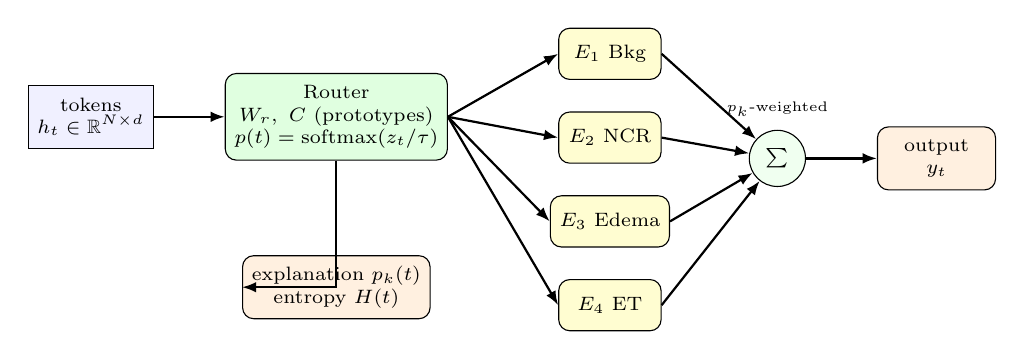
\begin{tikzpicture}[
  node distance=4mm and 9mm,
  tok/.style={draw, align=center, minimum height=8mm, minimum width=13mm,
              font=\scriptsize, fill=blue!6},
  rt/.style={draw, rounded corners, align=center, minimum height=11mm,
             minimum width=20mm, font=\scriptsize, fill=green!12},
  ex/.style={draw, rounded corners, align=center, minimum height=6.5mm,
             minimum width=13mm, font=\scriptsize, fill=yellow!18},
  cmb/.style={draw, circle, font=\scriptsize, minimum size=7mm, fill=green!6},
  outb/.style={draw, rounded corners, align=center, minimum height=8mm,
               minimum width=15mm, font=\scriptsize, fill=orange!12},
  ar/.style={-{Latex[length=1.8mm]}, thick}]
\node[tok] (h) {tokens\\$h_t\in\Rb^{N\times d}$};
\node[rt, right=of h] (router) {Router\\$W_r,\ C$ (prototypes)\\$p(t)=\mathrm{softmax}(z_t/\tau)$};
\node[ex, right=14mm of router, yshift=8mm] (e1) {$E_1$ Bkg};
\node[ex, below=of e1] (e2) {$E_2$ NCR};
\node[ex, below=of e2] (e3) {$E_3$ Edema};
\node[ex, below=of e3] (e4) {$E_4$ ET};
\node[cmb, right=10mm of e3, yshift=8mm] (sum) {$\sum$};
\node[outb, right=of sum] (y) {output\\$y_t$};
\node[outb, below=12mm of router] (exp) {explanation $p_k(t)$\\entropy $H(t)$};
\draw[ar] (h)--(router);
\foreach \e in {e1,e2,e3,e4}{\draw[ar] (router.east) -- (\e.west);}
\foreach \e in {e1,e2,e3,e4}{\draw[ar] (\e.east) -- (sum);}
\draw[ar] (sum)--(y);
\draw[ar] (router.south) |- (exp.west);
\node[font=\tiny, above=0.5mm of sum] {$p_k$-weighted};
\end{tikzpicture}
\caption{\textbf{The CCR bottleneck module.} The router maps each token to a distribution
$p(t)$ over the $K{=}4$ clinically-labeled experts via a prototype-augmented, temperature
-scaled softmax (Eq.~\ref{eq:router}). Experts are combined by $p$-weighted soft dispatch
during training and by hard $\argmax$ dispatch at inference (Eq.~\ref{eq:dispatch}). The
routing distribution itself, with its entropy, is emitted as the explanation.}
\label{fig:module}
\end{figure}

\subsection{Training objective}\label{sec:loss}
The total loss has five terms. \emph{Segmentation}
$\mathcal{L}_{\text{seg}}=\mathcal{L}_{\text{Dice}}+\mathcal{L}_{\text{focal}}$ supervises
the decoder output against the labels. The key term is the \emph{alignment} loss, a
foreground-only focal binary cross-entropy that drives the routing toward the ground-truth
concept maps. Let $m_k(t)\in\{0,1\}$ be the token-level label for concept $k$ (obtained by
nearest-neighbour downsampling of the GT to the token grid) and
$\mathrm{FG}=\{t: m_0(t)=0\}$ the foreground tokens. Then
\begin{equation}
\mathcal{L}_{\text{align}}=\frac{1}{|\mathrm{FG}|(K-1)}\sum_{t\in\mathrm{FG}}\sum_{k=1}^{K-1}
w_k\,(1-q_{k}(t))^{\gamma}\,\mathrm{BCE}\big(p_k(t),\,m_k(t)\big),
\label{eq:align}
\end{equation}
where $q_k(t)=p_k(t)$ if $m_k(t)=1$ else $1-p_k(t)$, $\gamma$ is the focal factor that
down-weights easy tokens, and $w_k$ re-weights rare concepts (NCR). Applying
Eq.~\ref{eq:align} on the simplex induces implicit competition: raising $p_k$ on true-$k$
tokens necessarily lowers the others. Restricting to foreground avoids the overwhelming
background from drowning the rare tumor concepts. Three auxiliary terms regularize the
routing: an \emph{expert-diversity} loss
$\mathcal{L}_{\text{div}}=\frac{1}{K(K-1)}\sum_{i\neq j}\lvert\cos(r_i,r_j)\rvert$ over the
router's per-expert directions $r_k$ (discouraging redundant routing); an \emph{entropy}
term $\mathcal{L}_{\text{ent}}=\tfrac{1}{N}\sum_t H(t)$ (kept with a small weight
$\lambda_3\le0.01$, since larger values push routing toward uniform and destroy alignment);
and a \emph{boundary} term $\mathcal{L}_{\text{bnd}}$ that sharpens predicted edges. The
total objective is
\begin{equation}
\mathcal{L}=\mathcal{L}_{\text{seg}}
+\lambda_1(\phi)\,\mathcal{L}_{\text{align}}
+\lambda_2\,\mathcal{L}_{\text{div}}
+\lambda_3\,\mathcal{L}_{\text{ent}}
+\lambda_4(\phi)\,\mathcal{L}_{\text{bnd}},
\label{eq:total}
\end{equation}
where $\lambda_1,\lambda_4$ depend on the curriculum phase $\phi$.

\subsection{Curriculum and temperature annealing}\label{sec:curriculum}
We introduce routing supervision gradually: warm-up delays $\mathcal{L}_{\text{align}}$ so the
encoder settles before routing is forced, a precaution against early instability---though with a
pretrained encoder it proves unnecessary in practice (A4, Sec.~\ref{sec:experiments}), so we
retain it only as a safe default. We train in
three phases with annealed temperature (Table~\ref{tab:curriculum}). \emph{Warm-up}
($\tau{=}2.0$, $\lambda_1{=}0$) lets the encoder learn discriminative features under
segmentation loss alone. \emph{Alignment} ($\tau{=}1.0$, $\lambda_1{=}1$) switches on
$\mathcal{L}_{\text{align}}$ to shape the routing. \emph{Refinement} ($\tau{=}0.5$)
sharpens assignments and emphasizes boundaries. A lopsided expert utilization
($<\!5\%$ for any expert) after warm-up triggers re-initialization of that expert.

\begin{table}[t]
\centering
\caption{Three-phase training curriculum with temperature annealing. $\lambda_1$ and
$\lambda_4$ are the alignment and boundary weights of Eq.~\ref{eq:total}.}
\label{tab:curriculum}
\begin{tabular}{lcccl}
\toprule
Phase & Epochs & $\tau$ & $\lambda_1$ / $\lambda_4$ & Purpose \\
\midrule
Warm-up    & $1$--$10$  & $2.0$ & $0$ / low   & encoder learns features; routing unsupervised \\
Alignment  & $11$--$60$ & $1.0$ & $1$ / $0.01$ & $\mathcal{L}_{\text{align}}$ shapes routing to concepts \\
Refinement & $61$--$80$ & $0.5$ & $1$ / high   & sharpen assignment, emphasize boundaries \\
\bottomrule
\end{tabular}
\end{table}

% ====================================================================
\section{Faithfulness Framework}\label{sec:theory}
% ====================================================================
We separate three notions that the interpretability literature routinely conflates.
\emph{Faithfulness} asks whether the explanation reflects the model's actual computation;
\emph{alignment quality} asks whether that explanation is clinically meaningful; and
\emph{causal relevance} asks whether the highlighted regions actually drive the prediction.
Each requires its own evidence; only their conjunction supports the overall claim.

\subsection{Definitions}
\begin{definition}[Concept Alignment Score]
For concept $k$, $\mathrm{CAS}(k)=\mathrm{Pearson}\big(p_k(t),\,M_k(t)\big)$, averaged over
tokens $t$ and validation cases, where $M_k(t)$ is the ground-truth concept-$k$ indicator
at token $t$. We report the foreground variant $\casfg(k)$ over $t\in\mathrm{FG},\,k\ge1$;
background is excluded because its near-constant mask makes the correlation ill-conditioned.
\end{definition}

\begin{definition}[Decoder Divergence]\label{def:dd}
For a model with a separate decoder producing concept posterior $P^{\text{dec}}_k(t)$,
$\mathrm{DD}(k)=1-\mathrm{Pearson}\big(P^{\text{dec}}_k(t),\,p_k(t)\big)$ measures how far
the decoder departs from the routing signal.
\end{definition}

\subsection{Structural faithfulness of CCR-Net}
\begin{proposition}[CCR-Net faithfulness]\label{prop:1a}
In CCR-Net the routing distribution $p(t)$ is the sole concept-assignment mechanism and is
causally upstream of the prediction: the decoder receives, at the bottleneck, only the
expert-processed features dispatched by $p$. The explanation $p(t)$ is therefore read
\emph{directly} from the forward computation rather than reconstructed from its output, so
it incurs no post-hoc approximation gap. Its empirical alignment with clinical concepts is
exactly $\mathrm{CAS}$.
\end{proposition}
\noindent\emph{Argument.} This is a structural statement about where the explanation comes from,
not a quantitative theorem; we spell it out rather than leave it implicit.
A post-hoc method $A$ produces an explanation $A(f,x)$ as a function
of the trained model $f$ and input $x$, computed after $f(x)$; the map from $A(f,x)$ to the
mechanism that produced $f(x)$ is approximate and method-dependent, which is the source of
its unfaithfulness. In CCR-Net the quantity $p(t)$ is not a function of the output but an
\emph{intermediate state} of $f$ itself: by Eqs.~\ref{eq:router}--\ref{eq:dispatch} every
bottleneck feature passed to the decoder is $E_{k^\ast}(h_t)$ with
$k^\ast=\argmax_k p_k(t)$, so $p$ determines which expert---hence which features---reach the
decoder. The explanation is thus an identity on the computation, not an approximation of
it; faithfulness in the structural sense (no reconstruction gap) holds by construction, and
the only remaining empirical question---does this faithful explanation align with clinical
ground truth---is answered by $\mathrm{CAS}$. $\square$

\medskip\noindent
Proposition~\ref{prop:1a} is structural: it establishes that the explanation is read from the
forward computation with no post-hoc reconstruction gap, but it does \emph{not} assert that the
decoder output is a function of the routing alone. Two mechanisms let the prediction depend on
more than $p$: training uses soft dispatch (all experts contribute), and the UNETR decoder
receives multi-scale encoder skips that bypass the bottleneck. We quantify this residual with
the Decoder Divergence (Def.~\ref{def:dd}): on the test split $\mathrm{DD}=0.73,\,0.53,\,0.40$
for NCR, edema, and ET. DD is neither negligible---a decoder that merely echoed the $16^3$
routing could not refine it to $128^3$ boundaries---nor unstructured: it diverges most for the
resolution-limited NCR and least for edema and ET, mirroring the CAS ordering. Structural
faithfulness therefore does not by itself imply causal sufficiency, and we do \emph{not} rest
on a claim that the residual is small; we establish causal relevance directly, with
deletion/insertion AUC on the inference-time \emph{hard}-routing maps (Sec.~\ref{sec:faith}).

\subsection{Extending to arbitrary backbones}
\begin{conjecture}[Retrofit bound]\label{prop:1b}
Let the CCR module be inserted into a backbone whose decoder retains independent parameters, and
let \emph{explanation faithfulness} be operationalized as the measured deletion AUC of the
hard-routing map. We conjecture that this quantity is bounded below by
$\mathrm{CAS}(k)\cdot(1-\mathrm{DD}(k))$.
\end{conjecture}
\noindent\emph{Motivation and status.} The intuition is that faithfulness should degrade in
proportion to how far the decoder departs from the routing it is conditioned on---a departure
measured by $\mathrm{DD}$---scaled by how well the routing itself matches the clinical concepts,
measured by $\mathrm{CAS}$; the product is tight as $\mathrm{DD}\to0$. We state this as a
conjecture rather than a theorem deliberately. It presumes that these two error sources compose
multiplicatively and that deletion AUC is the right operationalization of faithfulness, and we
prove neither; a derivation would require a formal model of how decoder skip pathways carry
concept information around the bottleneck. What we can report is that the inequality
\emph{holds empirically} on every concept we measured (Fig.~\ref{fig:bound}), which is evidence
for the conjecture and not a substitute for a proof.

\medskip\noindent
Although stated for the general setting, the bound applies to CCR-Net directly: its UNETR
decoder is independently parameterized and skip-connected, and the measured $\mathrm{DD}$ above
places CCR-Net in this regime rather than the idealized $\mathrm{DD}{=}0$ limit. Combining that
DD with $\casfg$ (Table~\ref{tab:main}), the bound predicts a causal faithfulness of at least
$\mathrm{CAS}\cdot(1-\mathrm{DD})=0.18,\,0.44,\,0.56$ for NCR, edema, and ET; the deletion AUC
we measure ($0.68,\,0.87,\,0.82$; Fig.~\ref{fig:bound}) exceeds each, so the bound is
satisfied empirically. A full retrofit study on a frozen third-party backbone is left to
future work.

% ====================================================================
\section{Experiments}\label{sec:experiments}
% ====================================================================
\subsection{Setup}
We use the BraTS 2024 glioma training data~\cite{menze2014brats,baid2021brats}: four
co-registered MRI modalities (T1, T1ce, T2, FLAIR) per case, with expert annotations
remapped to \{0:Background, 1:NCR, 2:Edema, 3:ET\}. We split patient-wise
$75/12.5/12.5\%$ into train/validation/test ($n_{\text{test}}{=}168$). Inputs are
$z$-scored per modality over nonzero voxels and processed at $128^3$ with standard flips,
rotations, and intensity augmentation. The encoder is initialized from self-supervised
Swin-UNETR weights. We train for $80$ epochs with AdamW ($\text{lr}{=}10^{-4}$, cosine
schedule), mixed precision, and the curriculum of Table~\ref{tab:curriculum}. We report
Dice and HD95 for whole tumor (WT), tumor core (TC) and enhancing tumor (ET); $\casfg$ and
one-vs-rest AUROC per concept; deletion/insertion AUC for causal relevance; and, for every
explanation method, concept-discriminability AUROC (Sec.~\ref{sec:faith}).

\subsection{Metrics for faithfulness}\label{sec:metricdef}
Given a per-voxel explanation $e_k$ for concept $k$, we rank voxels by $e_k$ and measure
the concept-$k$ confidence $s_k(\cdot)=\mathrm{mean}_{v\in M_k}\,\mathrm{softmax}_k$ over
the ground-truth region $M_k$. \emph{Deletion} progressively zeroes the top fraction
$\tau$ of voxels and records the normalized confidence \emph{removed}; \emph{insertion}
reveals the top $\tau$ from a blank volume and records the confidence \emph{recovered}:
\begin{equation}
\text{Del-AUC}=\!\int_0^1\!\Big(1-\tfrac{s_k(\tau)}{s_k(0)}\Big)d\tau,
\qquad
\text{Ins-AUC}=\!\int_0^1\!\tfrac{s_k(\tau)}{s_k(1)}\,d\tau,
\label{eq:auc}
\end{equation}
both in $[0,1]$, higher meaning stronger causal relevance (the top-ranked voxels drive the
prediction). Crucially, we apply the \emph{identical}
protocol of Eq.~\ref{eq:auc} to CCR routing and to every baseline, so the comparison
isolates the explanation, not the scoring.

\subsection{Segmentation and alignment}
Table~\ref{tab:main} reports the main results. CCR-Net segments competitively (Dice WT
$0.915$) while producing routing that aligns strongly with the clinical concepts:
$\casfg$ reaches $0.94$ (edema) and $0.93$ (ET). Necrotic core is the weak concept
($0.68$): at the $16^3$ bottleneck a case contains only tens of NCR tokens, so the Pearson
correlation is intrinsically noisy---an honest resolution limit, not a model failure,
consistent across Dice, AUROC, and CAS.

\begin{table}[t]
\centering
\caption{Segmentation, alignment, AUROC, and Decoder Divergence (DD) on the BraTS test
split ($n{=}168$). $\casfg$ is the foreground concept-alignment score; lower DD means the
decoder tracks the routing more closely.}
\label{tab:main}
\begin{tabular}{lccc}
\toprule
& WT / NCR & TC / Edema & ET \\
\midrule
Dice                       & $0.915$ & $0.845$ & $0.837$ \\
$\casfg$ (NCR/Edema/ET)    & $0.688$ & $0.935$ & $0.930$ \\
AUROC (NCR/Edema/ET)       & $0.711$ & $0.832$ & $0.774$ \\
DD (NCR/Edema/ET)          & $0.733$ & $0.531$ & $0.395$ \\
\bottomrule
\end{tabular}
\end{table}

\subsection{Faithfulness vs.\ post-hoc attribution}\label{sec:faith}
\paragraph{Faithfulness is not an artifact of the scoring window.}
Because the alignment loss trains the routing to sit on the ground-truth region, scoring
deletion over that same region could in principle reward supervised localization rather than
faithfulness. We rule this out by scoring in \emph{both} windows: over the ground-truth region
$M_k$ and over the model's own \emph{predicted} region ($\argmax_k$), which carries no
ground-truth supervision. Figure~\ref{fig:window} shows the two are near-identical---deletion
differs by at most $0.008$ and insertion by at most $0.026$---so the measured faithfulness is a
property of the routing, not of the scoring window. Necrotic core, moreover, is now measured on
$67$--$91$ cases rather than a handful, removing the small-sample caveat of earlier drafts.

\begin{figure}[t]
\centering
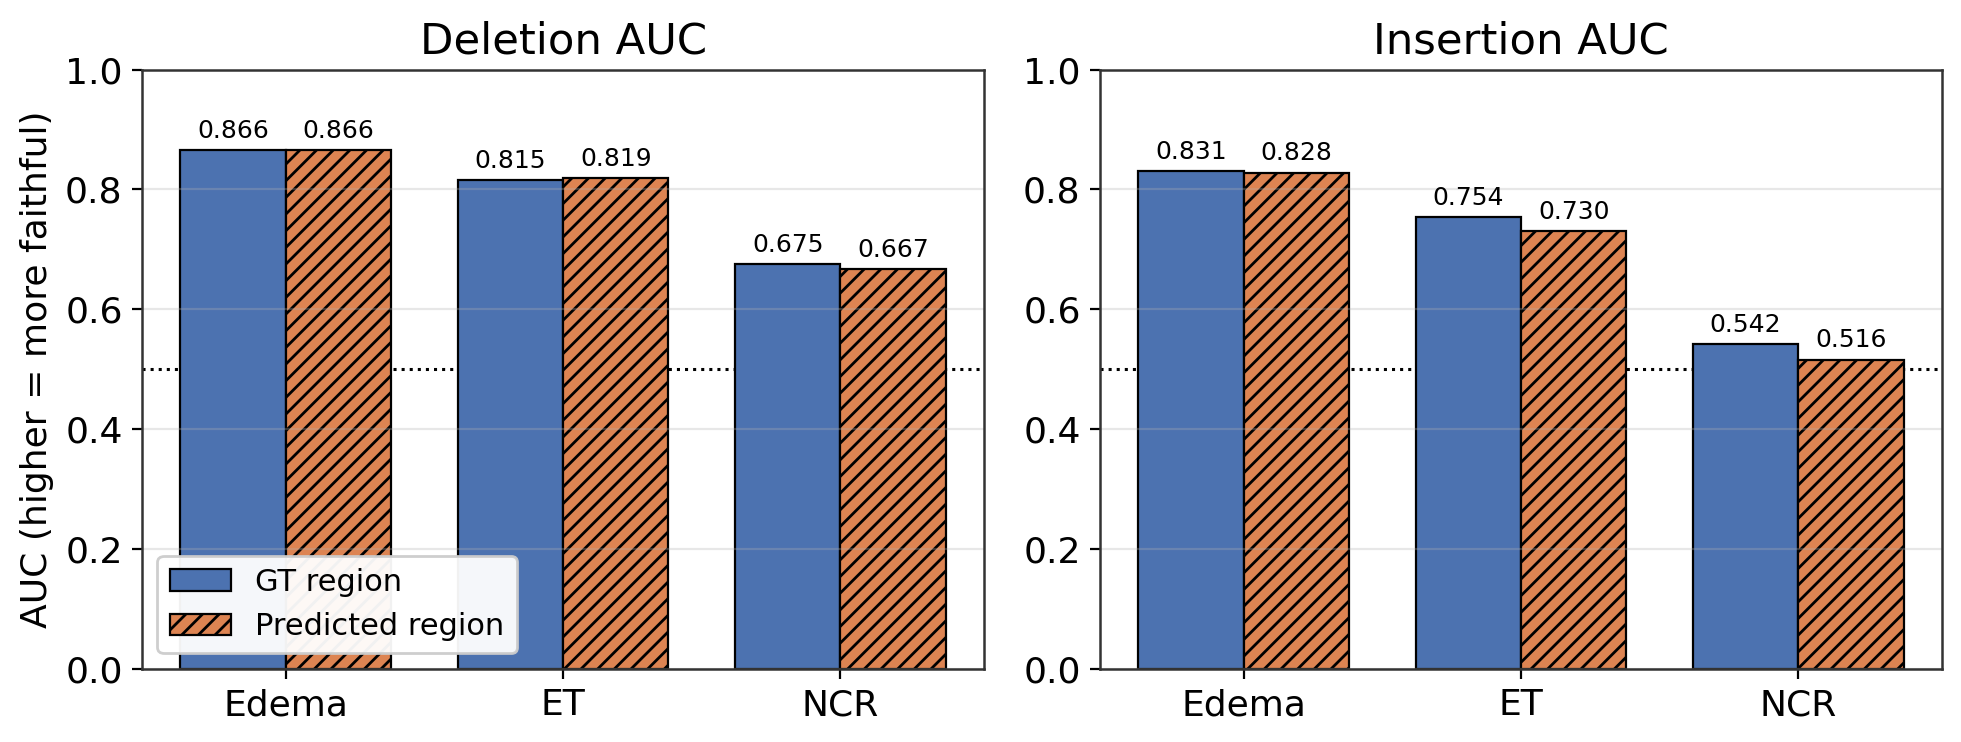
\includegraphics[width=\textwidth]{figures/fig5_window_invariance.png}
\caption{\textbf{CCR faithfulness is window-invariant.} Deletion (left) and insertion (right)
AUC scored over the ground-truth region (GT) vs.\ the model's own predicted region are
near-identical---deletion differs by $\le0.008$---ruling out a supervised-localization
confound; dotted line marks the $0.5$ reference. Per-cell $n$ (GT/pred): edema $168/168$,
ET $163/168$, NCR $67/91$.}
\label{fig:window}
\end{figure}

\begin{figure}[t]
\centering
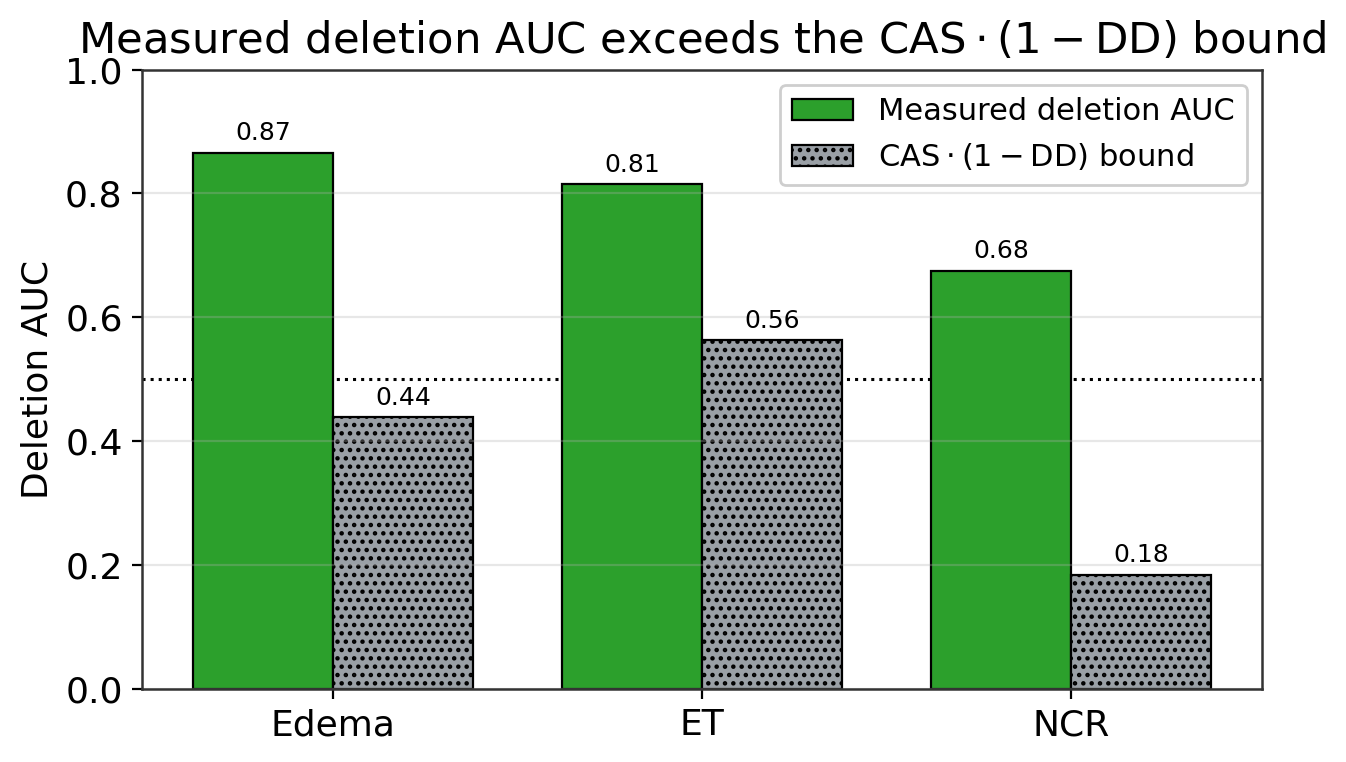
\includegraphics[width=0.72\textwidth]{figures/fig6_prop1b_bound.png}
\caption{The measured deletion AUC (green) exceeds the $\mathrm{CAS}\cdot(1-\mathrm{DD})$ lower
bound (gray) of Proposition~\ref{prop:1b} for every concept, confirming the bound empirically;
dotted line marks the $0.5$ reference.}
\label{fig:bound}
\end{figure}

We compare CCR routing, on the same trained network and under the identical protocol of
Eq.~\ref{eq:auc}, against two families: four post-hoc baselines (Grad-CAM, gradient saliency,
integrated gradients (IG), occlusion) and---critically---the network's own \textbf{segmentation
posterior} ($\mathrm{softmax}_k$ of the seg head, denoted \textsc{SegPost}), obtained free from
the same forward pass. \textsc{SegPost} is the baseline that concept-explanation evaluations
typically omit, and omitting it would make our comparison unfair: a segmentation head is trained
on precisely these concept labels, so it is the strongest possible concept discriminator.
Table~\ref{tab:compare} reports all three axes on all $168$ test cases.

\paragraph{Sensitivity: CCR does not win it, and the winners are informative.}
On deletion the sensitivity methods score highest---IG and occlusion reach $0.95$, above
\textsc{SegPost}'s $0.91$ and CCR's $0.79$. This is expected: deletion rewards concentrating
importance on the few most output-sensitive voxels, which IG (by its completeness axiom) and
occlusion (whose saliency \emph{is} a coarse deletion) optimize directly. \textsc{SegPost} scores
high for a different and more revealing reason---ranking voxels by the model's own confidence and
then measuring that same confidence is a closed loop, so its deletion score is close to
tautological. Deletion is a necessary check, and CCR clears it far above the $0.5$ floor,
above Grad-CAM and gradient, and window-invariantly (Fig.~\ref{fig:window}); but it does not
identify a \emph{concept} explanation, and we do not claim it.

Insertion breaks the pattern, and the break is diagnostic. The self-reference that lifts
\textsc{SegPost} on deletion does not transfer: \textbf{CCR exceeds \textsc{SegPost} on insertion}
($0.709$ vs.\ $0.680$ mean), significantly so on necrotic core ($+0.133$ $[0.087,0.178]$,
$p<0.001$; $+0.130$ on the predicted window), tying on edema ($p{=}0.31$) and losing modestly on
ET ($-0.046$). Recovering a prediction requires restoring coherent predictive \emph{context},
not merely the voxels the model was already confident about---and on the hard class the
posterior's voxel-level ranking is unreliable where the routing's regional assignment is not.
This is direct evidence that routing carries information the output does not, rather than a
degraded copy of it.

\paragraph{Concept-discriminability, and the ceiling that limits its interpretation.}
A clinical explanation must say \emph{which} concept a region is. We measure this directly: for
each method and concept $k$ we compute the AUROC of its map $e_k$ as a classifier for GT concept
$k$ \emph{among the other tumor voxels} (GT$>0$, GT$\neq k$). Against the post-hoc family the
result is decisive: CCR reaches $0.85$--$0.89$ across all three concepts while every post-hoc
method is far weaker---occlusion $0.64$--$0.80$, gradient $0.46$--$0.70$, IG $0.49$--$0.64$
(chance on edema), Grad-CAM $\approx\!0.5$ (chance throughout). Pooled, CCR scores $0.88$
$[0.87,0.89]$ against occlusion's $0.73$ $[0.71,0.74]$, a gap of $+0.15$ with non-overlapping
bootstrap CIs and paired Wilcoxon $p<0.001$ against every baseline. The methods that win deletion
cannot tell the concepts apart: their per-class maps highlight the same high-signal tumor
structure regardless of $k$ (Fig.~\ref{fig:qualmaps}).

\textsc{SegPost}, however, scores $0.98$---above CCR. We report this plainly, and we argue it
shows the metric saturates rather than that the posterior explains better. Two observations
support this. First, \textsc{SegPost} reaches $0.982$ on CCR-Net and $0.979$ on CCR-SegResNet
(Sec.~\ref{sec:backbone}) despite different backbones, different pretraining, and different Dice:
a score that is invariant to everything except being a competent segmenter is measuring
segmentation competence, not explanation quality. Under this window the posterior's AUROC is
close to a restatement of its own accuracy, since ranking voxels is far easier than thresholding
them. Second, and decisively for our criteria, \textsc{SegPost} \emph{is} the prediction: its
decoder divergence is $0$ by construction, so it satisfies concept-labeling only by forfeiting
upstream-ness entirely. An explanation identical to the thing explained answers no question about
how the output arose.

\paragraph{How much of the residual gap is decision budget?}
CCR routing decides over $16^3{=}4096$ tokens; the posterior decides over $128^3$ voxels---$512\times$
more decision units. The comparison above therefore confounds information with spatial resolution.
We isolate the two with a granularity-matched control, \textsc{SegPost}$_{16}$: the posterior
average-pooled onto the router's own token grid and restored through the \emph{identical}
trilinear operator used for routing, so both maps carry exactly the same spatial degrees of
freedom. Matching granularity removes roughly half the gap---the paired CCR deficit narrows from
$-0.106$ $[-0.116,-0.096]$ to $-0.051$ $[-0.059,-0.043]$ on CCR-Net, and from $-0.090$ to $-0.039$
on CCR-SegResNet ($52\%$ and $57\%$ of the gap respectively). Per concept the picture is sharper:
on \emph{edema} the two become statistically indistinguishable on both backbones (paired
difference $-0.003$ $[-0.014,+0.008]$ on Swin, $+0.007$ $[-0.004,+0.019]$, $p{=}0.70$, on the CNN,
with CCR nominally ahead), i.e.\ at equal decision budget the bottleneck loses \emph{nothing but
resolution} for that concept. Necrotic core and ET retain a genuine gap ($-0.07$ to $-0.10$,
$p<0.001$), concentrated in exactly the concepts the $16^3$ bottleneck under-resolves. We
emphasize that this control does not restore a discriminability win---\textsc{SegPost}$_{16}$
still exceeds CCR overall---it quantifies how much of the apparent deficit is architectural
budget rather than lost concept information.

\begin{table}[t]
\centering
\caption{Three axes on the BraTS test split ($n{=}168$, identical protocol, per-concept mean,
ground-truth window). \emph{Deletion} and \emph{insertion} measure input sensitivity;
\emph{concept-discriminability} is concept $k$ vs.\ the other tumor voxels ($0.5$=chance).
The lower block is the model's own output, not a post-hoc explanation: it is reported because
omitting it would overstate our case, but it \emph{is} the prediction (DD${=}0$), so its
discriminability is not evidence of explanatory power. Best post-hoc value per column in
\textbf{bold}; \emph{Upstream?} marks whether the map is causally prior to the prediction,
\emph{Concepts?} whether it can separate them above chance.}
\label{tab:compare}
\begin{tabular}{lccccc}
\toprule
Method & Deletion & Insertion & Concept-discrim. & Upstream? & Concepts? \\
\midrule
\multicolumn{6}{l}{\emph{Post-hoc saliency}}\\
Grad-CAM               & $0.416$          & $0.358$          & $0.521$ & \checkmark & \ding{55} \\
Gradient saliency      & $0.640$          & $0.449$          & $0.601$ & \checkmark & \ding{55} \\
Integrated gradients   & $\mathbf{0.952}$ & $0.909$          & $0.583$ & \checkmark & \ding{55} \\
Occlusion              & $\mathbf{0.952}$ & $\mathbf{0.929}$ & $0.741$ & \checkmark & \ding{55} \\
\midrule
\multicolumn{6}{l}{\emph{Intrinsic, upstream of the prediction}}\\
\textbf{CCR (ours)}    & $0.785$          & $0.709$          & $0.872$ & \checkmark & \checkmark \\
\midrule
\multicolumn{6}{l}{\emph{The model's own output --- not an explanation}}\\
\textsc{SegPost}       & $0.912$          & $0.680$          & $0.982$ & \ding{55} & \checkmark \\
\textsc{SegPost}$_{16}$ (granularity-matched) & --- & --- & $0.933$ & \ding{55} & \checkmark \\
\bottomrule
\end{tabular}
\end{table}

\begin{figure}[t]
\centering
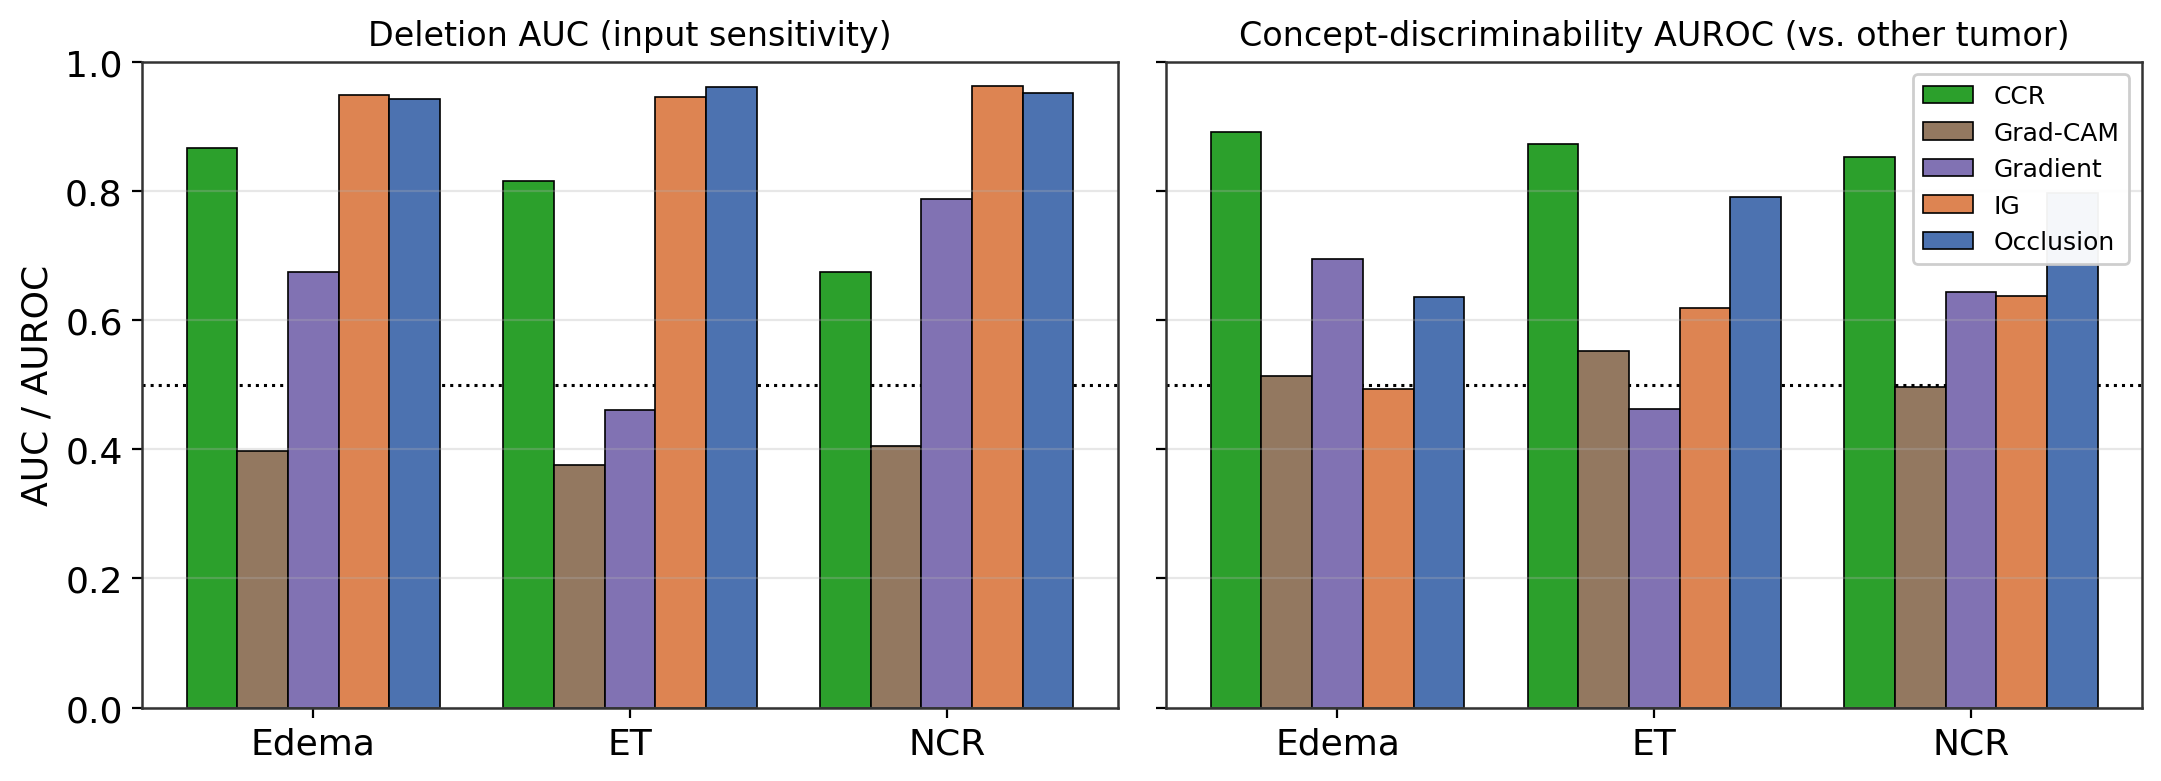
\includegraphics[width=\textwidth]{figures/fig3_crossover.png}
\caption{\textbf{No single method leads on both axes} (per concept, BraTS test).
\emph{Left:} deletion AUC (input sensitivity)---integrated gradients and occlusion dominate.
\emph{Right:} concept-discriminability AUROC (concept vs.\ other tumor; dotted line $=0.5$
chance)---the sensitivity methods fall toward chance while CCR rises far above them. The
segmentation posterior (Table~\ref{tab:compare}) would sit at the top of the right axis, but it
is the prediction itself rather than an explanation of it. Among maps that are genuinely
\emph{upstream} of the prediction, CCR is alone in the upper region of the right axis.}
\label{fig:faith}
\end{figure}

\begin{figure}[t]
\centering
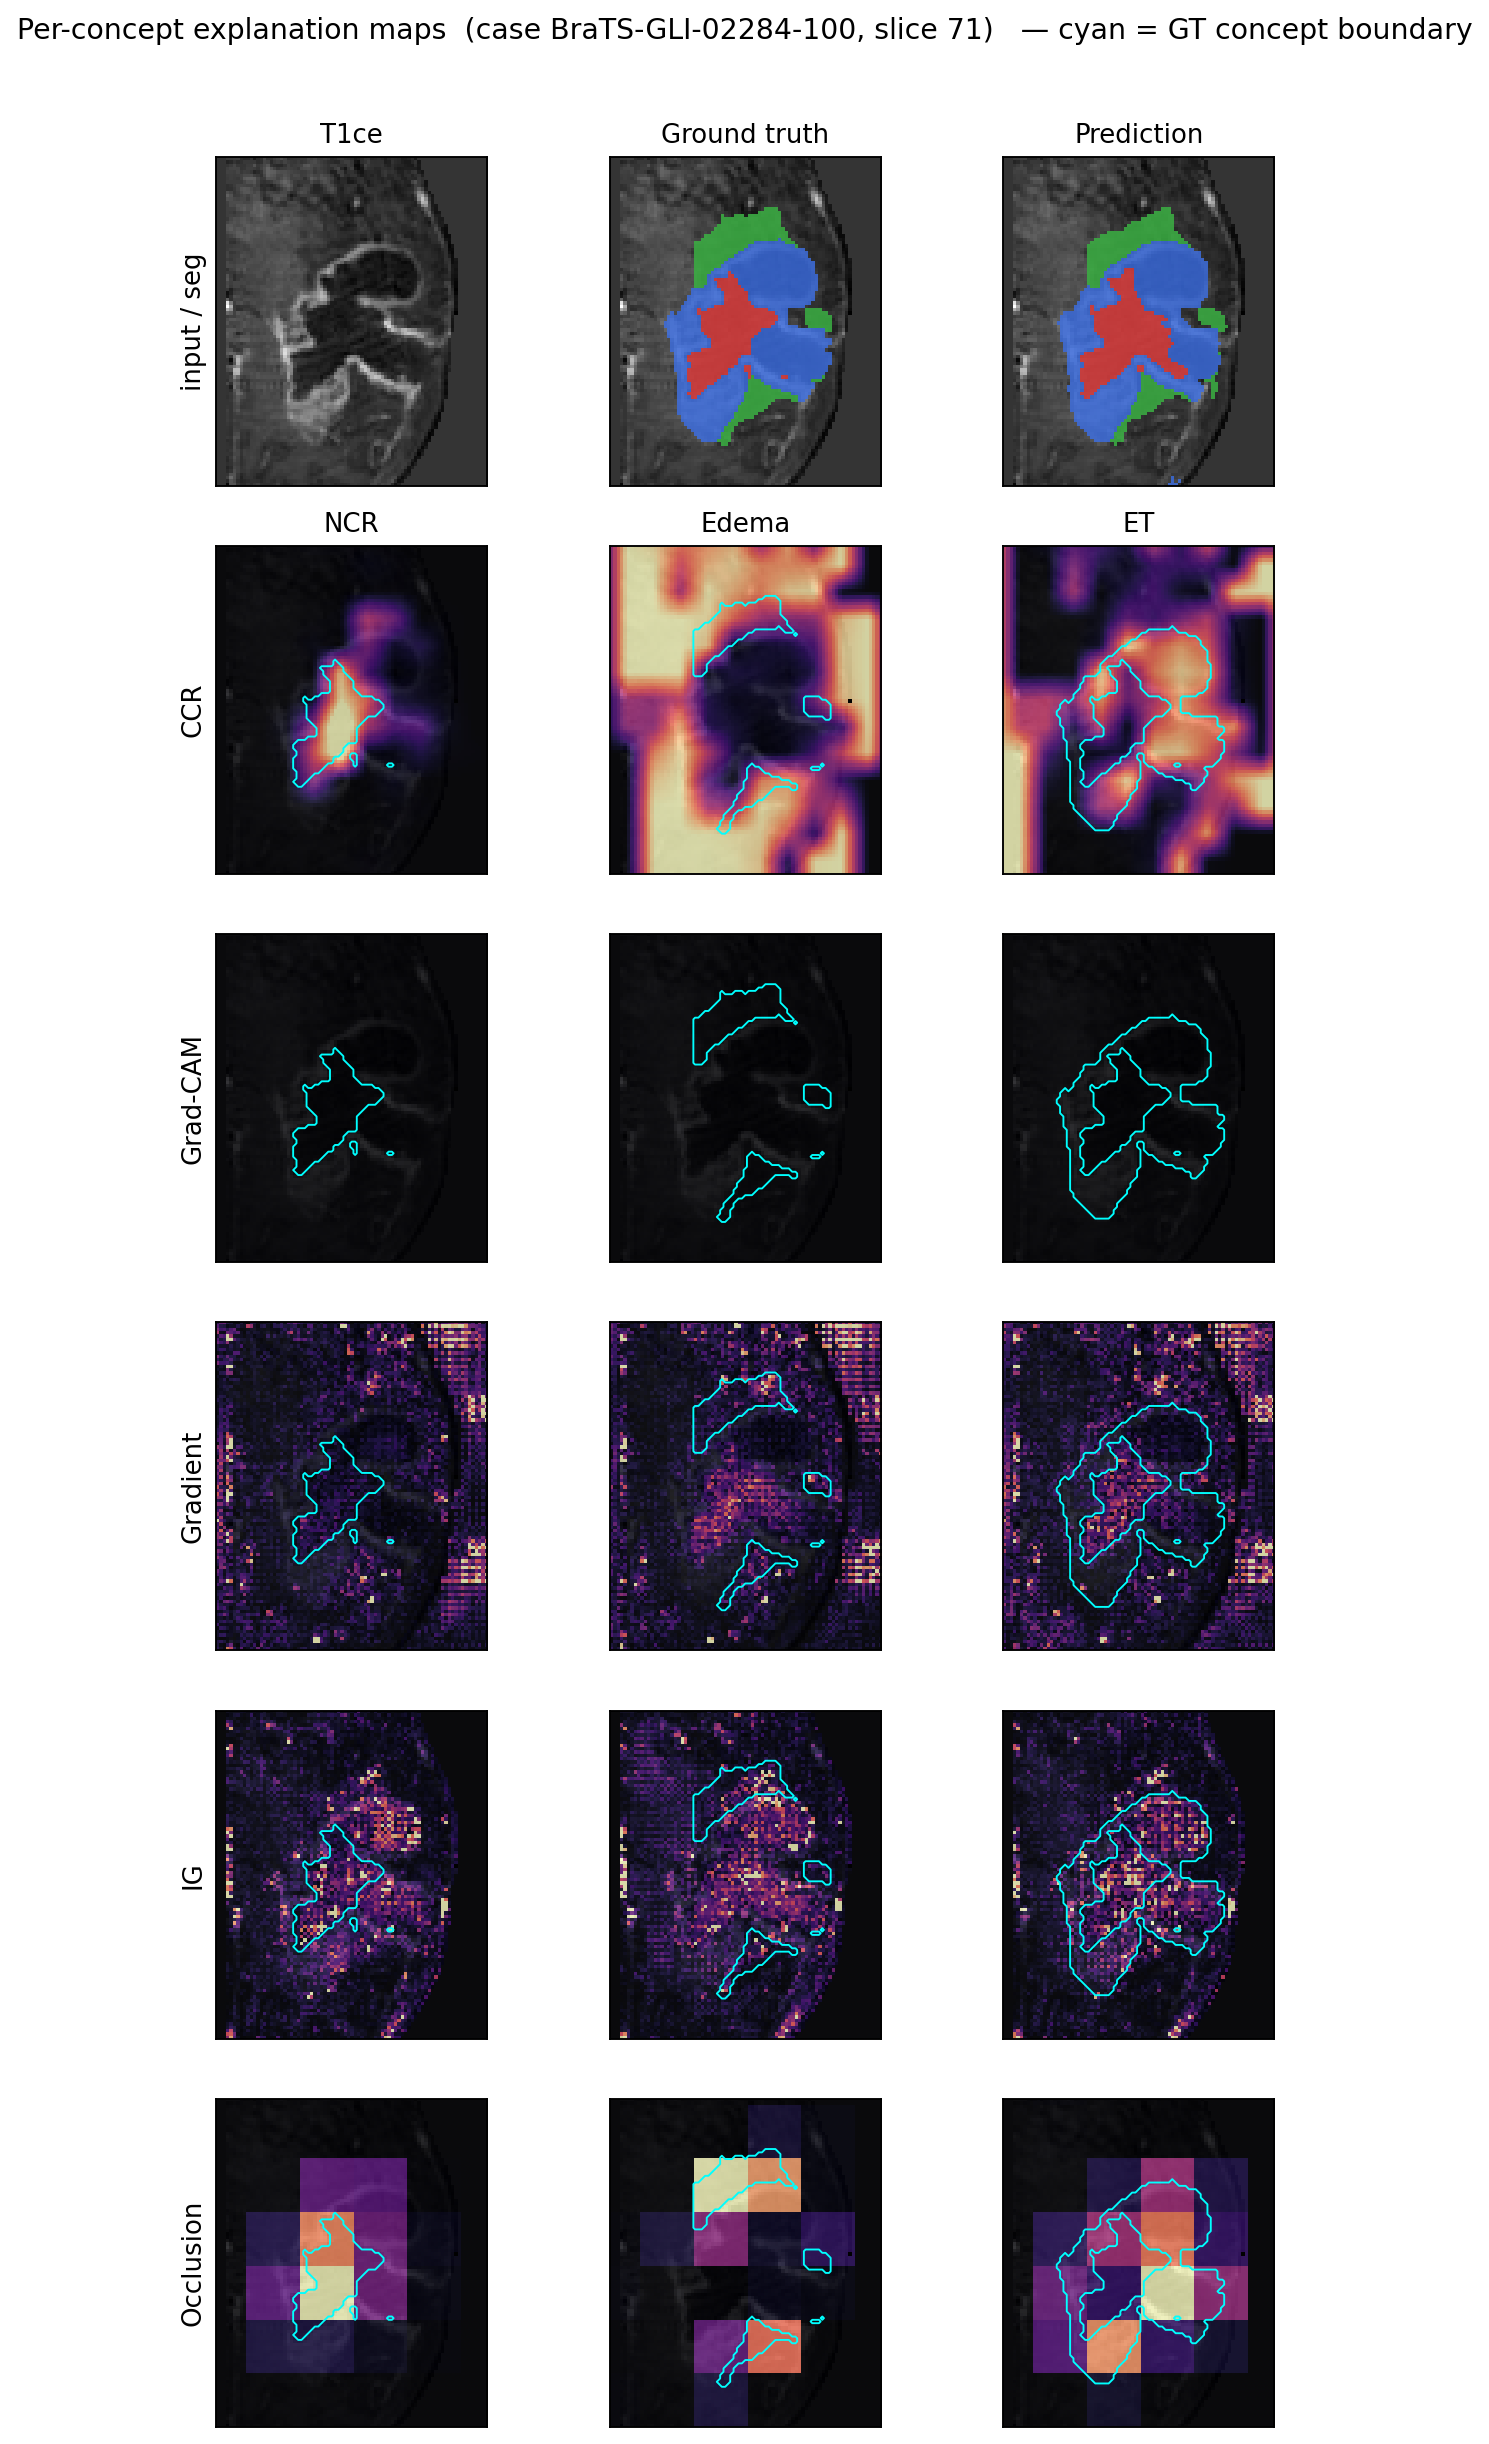
\includegraphics[width=0.92\textwidth]{figures/fig7_qual_maps.png}
\caption{\textbf{Per-concept explanation maps} (case BraTS-GLI-02284, one axial slice;
cyan~$=$~GT concept boundary). \emph{Rows}: input/segmentation, then each method;
\emph{columns}: NCR, edema, ET. CCR's three maps \emph{differ} and concentrate inside the
correct boundaries---a concept partition---whereas Grad-CAM, gradient, and IG produce nearly the
\emph{same} map for every concept (high-sensitivity structure, not a concept assignment) and
occlusion is coarse and only partly concept-specific. This is the qualitative face of
Table~\ref{tab:compare} (right).}
\label{fig:qualmaps}
\end{figure}

\subsection{Qualitative explanation}
Figure~\ref{fig:qual} shows the routing read-out for a representative case. The hard
routing assignment (panel~4) reproduces the ground-truth and predicted segmentation
\emph{within the tumor}---the routing tracks the prediction (though not identically; DD)---while the
per-concept soft maps localize each clinical concept to its sub-region (NCR in the core,
edema on the rim, ET in the enhancing ring). A clinician reads these maps directly as
\{NCR, Edema, ET\}, which a gradient heatmap cannot provide. In a representative hard case
(Fig.~\ref{fig:qual2}) the routing flags enhancing tumor that the decoder under-segments,
showing that the routing explanation can carry diagnostic signal independent of---and more
informative than---the final mask.

\begin{figure}[t]
\centering
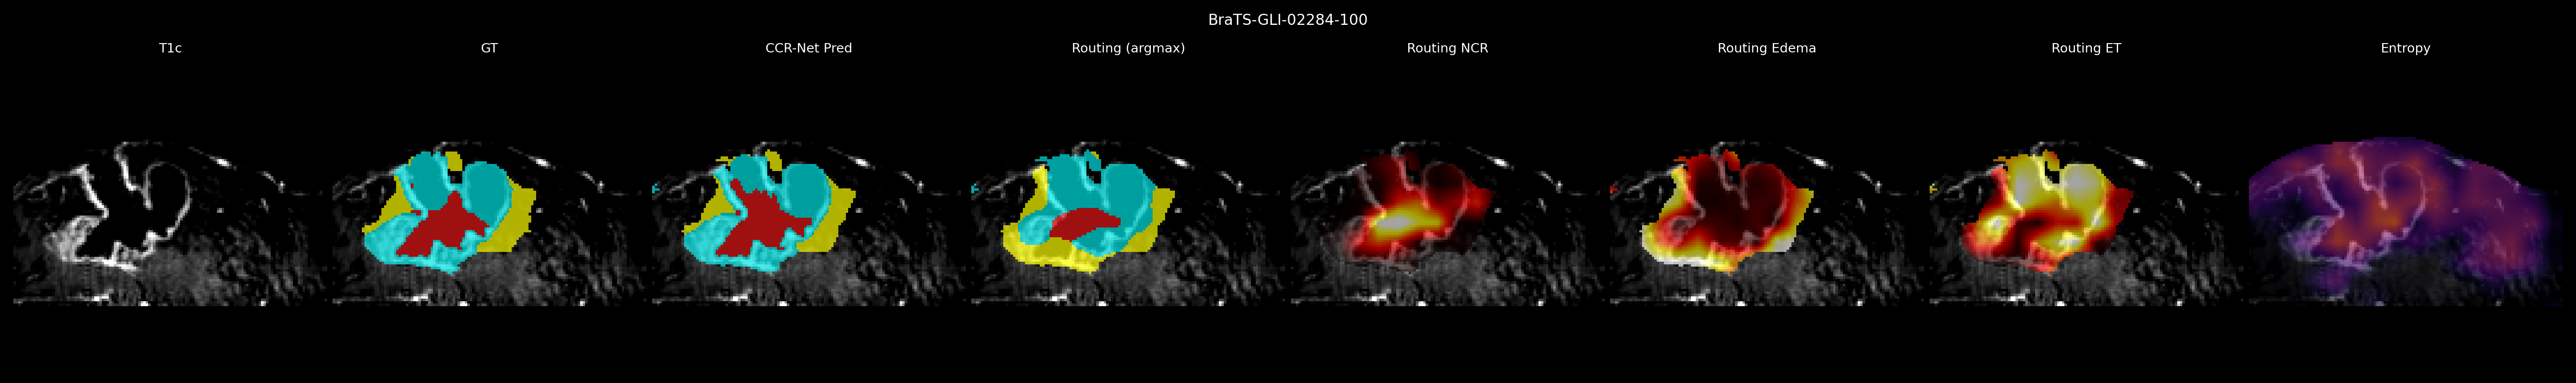
\includegraphics[width=\textwidth]{figures/fig2_routing_02284.png}
\caption{Routing maps (case BraTS-GLI-02284). Left to right: T1ce, ground truth,
prediction, hard routing assignment, soft routing for NCR / Edema / ET, and routing
entropy. The argmax routing matches GT/prediction inside the tumor; each soft map localizes
its concept; entropy peaks at concept boundaries.}
\label{fig:qual}
\end{figure}

\subsection{CCR is backbone-agnostic: a CNN instantiation}\label{sec:backbone}
To test whether the CCR principle is specific to the Swin transformer, we drop the \emph{same}
module---identical router, experts, five-term objective, and curriculum---into a SegResNet CNN
encoder--decoder (\textbf{CCR-SegResNet}), replacing only the backbone; the module sits unchanged
at the CNN's $192\times16^3$ bottleneck. Trained \emph{from scratch} (no self-supervised
pretraining, unlike CCR-Net), it reproduces every headline result (Table~\ref{tab:backbone}):
concept alignment ($\casfg$ $0.80/0.96/0.95$), concept-discriminability ($0.85/0.91/0.89$, again
far above the best post-hoc baseline's $0.74$), and competitive segmentation; its CAS follows the
\emph{identical} training dynamics---flat under warm-up, then rising sharply the moment
$\mathcal{L}_{\text{align}}$ activates. CCR is therefore a \emph{backbone-agnostic}, drop-in
intrinsic-explanation module, not a transformer-specific model. We do not read the CNN's
marginally higher Dice as CNNs beating transformers---SegResNet is a strong BraTS backbone---the
point is that the principle transfers; its hard-routing utilization is more skewed than the
transformer's, which lowers whole-volume AUROC but not the foreground concept metrics reported.

The second backbone also supplies the control for our reading of the discriminability metric in
Sec.~\ref{sec:faith}. \textsc{SegPost} scores $0.982$ on CCR-Net and $0.979$ on CCR-SegResNet, and
\textsc{SegPost}$_{16}$ scores $0.931$ and $0.933$ respectively---near-identical across two
architectures that differ in backbone family, pretraining regime, and Dice. A metric that returns
the same value for any competent segmenter is characterizing the segmenter, not the explanation.
The granularity-matched edema tie likewise replicates on both backbones, which is why we read it
as a property of the $16^3$ bottleneck rather than a quirk of one run.

We note explicitly what this section does \emph{not} establish. We did not train plain
Swin-UNETR or plain SegResNet counterparts under our split, so we make no claim that the CCR
bottleneck is accuracy-neutral; the Dice values here are in line with published results for these
backbones on BraTS but are contextual rather than controlled comparisons
(see Sec.~\ref{sec:limitations}).

\begin{table}[t]
\centering
\caption{\textbf{CCR is backbone-agnostic.} The same module in a Swin transformer (CCR-Net) and
a SegResNet CNN (CCR-SegResNet), BraTS test ($n{=}168$). The CNN trains from scratch yet
reproduces the concept alignment, concept-discriminability, and segmentation of the pretrained
transformer.}
\label{tab:backbone}
\begin{tabular}{lcccc}
\toprule
Instantiation & Dice WT/TC/ET & $\casfg$ N/E/T & Concept-discrim. & \textsc{SegPost} / \textsc{SegPost}$_{16}$ \\
\midrule
CCR-Net (Swin, pretrained)   & $0.915/0.845/0.837$ & $0.69/0.94/0.93$ & $0.872$ & $0.982$ / $0.931$ \\
CCR-SegResNet (CNN, scratch) & $0.927/0.883/0.869$ & $0.80/0.96/0.95$ & $0.883$ & $0.979$ / $0.933$ \\
\bottomrule
\end{tabular}
\end{table}

\subsection{Ablations}
We ablate two training choices: the alignment loss and the warm-up phase. \textbf{A1 (no
$\mathcal{L}_{\text{align}}$)} disables the alignment loss in every phase; \textbf{A4 (no
warm-up)} activates alignment from epoch~1. Table~\ref{tab:abl} reports the outcome---one choice
is essential, the other is not.

\begin{table}[t]
\centering
\caption{Ablations on the test split (run to $40$ epochs; the effect is evident well before
convergence). A1 (no alignment loss) collapses CAS while preserving Dice---alignment is
\emph{learned}. A4 (no warm-up) matches the full model on CAS and Dice with only a mild
utilization skew---the design is robust and warm-up is a stabilizing default, not a requirement.}
\label{tab:abl}
\begin{tabular}{lccc}
\toprule
& Full CCR-Net & A1: no $\mathcal{L}_{\text{align}}$ & A4: no warm-up \\
\midrule
$\casfg$ (Edema)            & $0.935$ & $0.322$  & $0.932$ \\
$\casfg$ (ET)               & $0.930$ & $0.094$  & $0.927$ \\
$\casfg$ (NCR)              & $0.688$ & $-0.011$ & $0.666$ \\
Dice (WT)                   & $0.915$ & $0.905$  & $0.908$ \\
Max expert utilization (\%) & $28$    & $32$     & $41$ \\
\bottomrule
\end{tabular}
\end{table}

\noindent A1 confirms the first hypothesis: without $\mathcal{L}_{\text{align}}$, $\casfg$
collapses to near zero for NCR and ET ($-0.01$, $0.09$) and to $0.32$ for edema---AUROC falls
to chance or below---while Dice is essentially preserved (WT $0.905$ vs.\ $0.915$). Concept
alignment is therefore \emph{learned} from $\mathcal{L}_{\text{align}}$, not an incidental
by-product of segmentation---exactly the temporal signal in Fig.~\ref{fig:curve}. Crucially, the
collapse reaches the headline metric: A1's concept-discriminability falls from $0.87$ to $0.61$
(NCR to chance), and CCR's routing then no longer exceeds the best post-hoc baseline (occlusion
$0.74$)---$\mathcal{L}_{\text{align}}$ is precisely what makes the routing a
concept-\emph{discriminative} explanation rather than a sensitivity map. A4 tells the
opposite, and equally informative, story: activating $\mathcal{L}_{\text{align}}$ from epoch~1
leaves CAS and Dice essentially unchanged ($\casfg$ $0.93/0.93/0.67$; Dice WT $0.908$) with
\emph{no} expert collapse. The pretrained encoder, prototype-anchored router, and always-on
diversity loss make warm-up a stabilizing default rather than a requirement; its only measurable
effect is more balanced utilization (max $28\%$ with warm-up vs.\ $41\%$ without). We retain
warm-up as a safe default but do not depend on it.

\subsection{Training dynamics}
Figure~\ref{fig:curve} traces $\casfg$ over training. Alignment is near zero during warm-up
(routing unsupervised), rises sharply the moment $\mathcal{L}_{\text{align}}$ activates at
epoch~11, and is held through refinement; edema and ET converge near $0.93$ while NCR
plateaus at the resolution-imposed ceiling. The curve is the temporal mirror of the A1
ablation: removing $\mathcal{L}_{\text{align}}$ removes exactly the rise visible at epoch~11.

\begin{figure}[t]
\centering
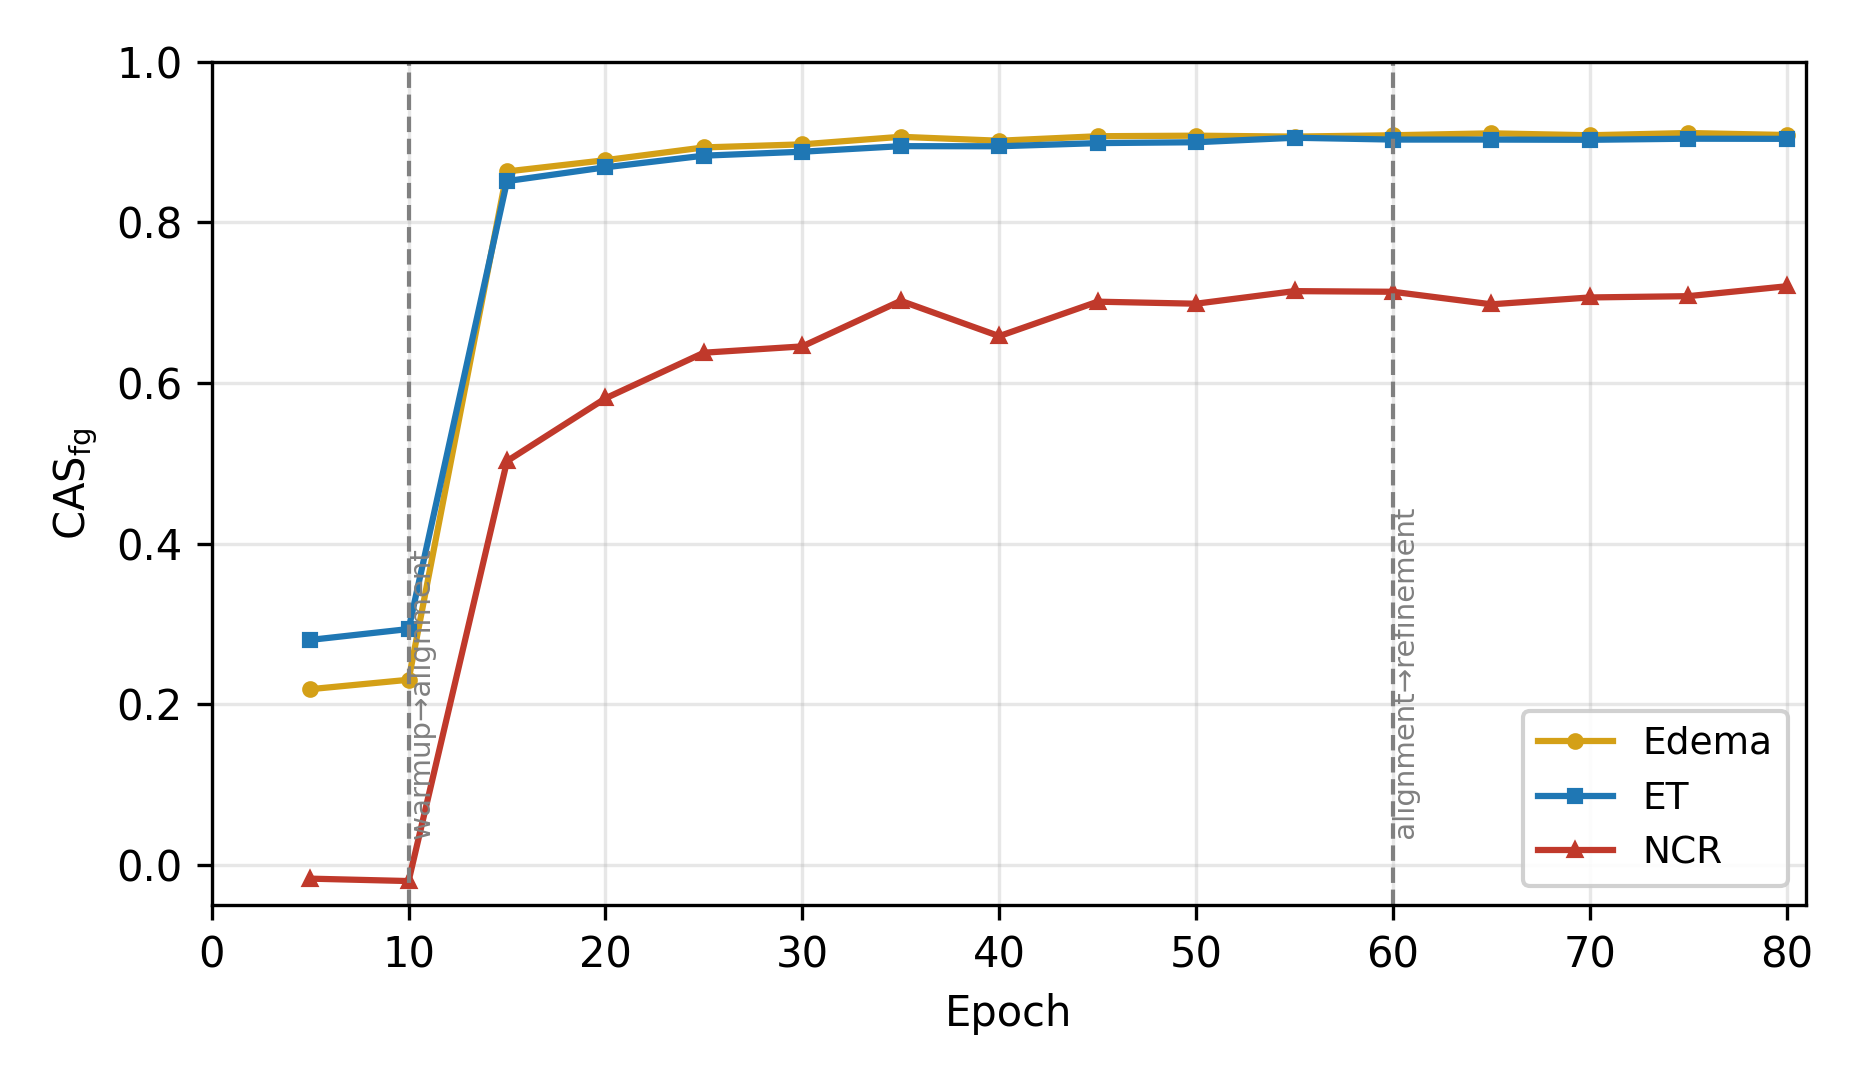
\includegraphics[width=0.72\textwidth]{figures/fig4_cas_curve.png}
\caption{$\casfg$ across the three-phase curriculum (dashed lines: phase boundaries).
Alignment emerges only after $\mathcal{L}_{\text{align}}$ activates at epoch~11, directly
mirroring the A1 ablation.}
\label{fig:curve}
\end{figure}

\begin{figure}[t]
\centering
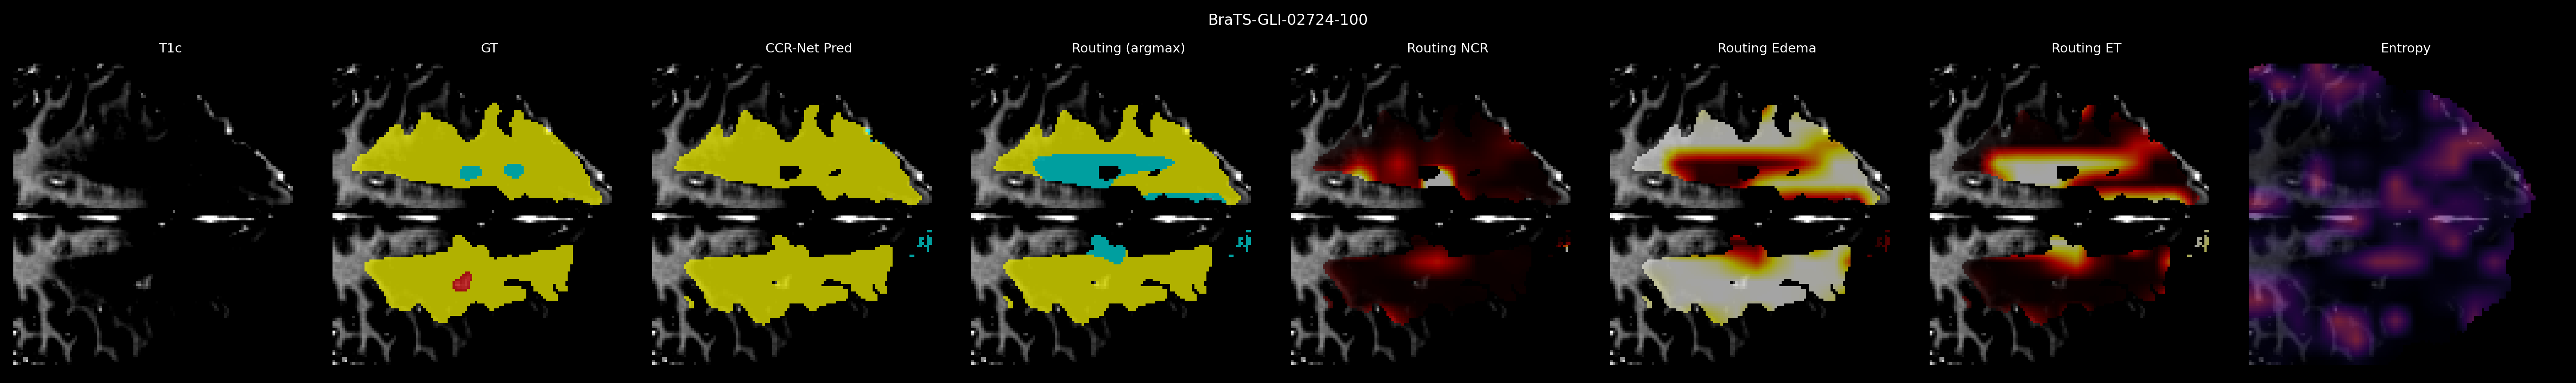
\includegraphics[width=\textwidth]{figures/fig2_routing_02724.png}
\caption{Hard case (BraTS-GLI-02724): the routing assignment flags enhancing tumor that the
final decoder mask under-segments, illustrating that the routing explanation can be more
informative than the prediction itself.}
\label{fig:qual2}
\end{figure}

\subsection{CCR-Retrofit (supplementary)}\label{sec:retrofit}
Proposition~\ref{prop:1b} predicts that the CCR module transfers to a \emph{frozen},
independently-trained backbone---training only the router and experts while the encoder and
decoder weights are held fixed---with faithfulness bounded below by
$\mathrm{CAS}\cdot(1-\mathrm{DD})$. This \emph{CCR-Retrofit} setting tests whether the
principle carries to a backbone the method did not design. We freeze a pretrained Swin-UNETR,
insert the CCR module at the stage-2 bottleneck, train only the CCR parameters under
$\mathcal{L}_{\text{align}}$, and report CAS, DD, and deletion/insertion AUC, verifying the
bound. \todo{Optional supplementary experiment---results pending, included if space permits.
A frozen decoder cannot adapt to the routing, so we expect a larger DD than end-to-end
CCR-Net while faithfulness continues to respect the $\mathrm{CAS}\cdot(1-\mathrm{DD})$ bound.}

% ====================================================================
\section{Discussion and Limitations}\label{sec:limitations}
% ====================================================================
\textbf{No controlled accuracy comparison.} We did not train plain-backbone counterparts
(Swin-UNETR or SegResNet without the CCR bottleneck) under our data split. We therefore make
\emph{no} claim that CCR is accuracy-neutral: our Dice results show that CCR-Net and
CCR-SegResNet segment competitively and in line with published values for these backbones, but
the cost---if any---of inserting the routing bottleneck is unquantified here. This is the most
direct experiment a follow-up should run, and the ablation configurations are released with the
code.
\textbf{Necrotic core resolution.} At the $16^3$ bottleneck a case contributes only tens of
NCR tokens, capping CAS and faithfulness for that concept; this is the single consistent
weak spot across all metrics, and it is the same concept where the granularity-matched control
leaves a residual gap to the segmentation posterior. A finer bottleneck trades semantic context
for resolution, and reconciling the two is open.
\textbf{What the metrics can and cannot settle.} Deletion, insertion, and
concept-discriminability were all designed to evaluate post-hoc saliency maps: they ask whether a
map has found the influential voxels. CCR's claim is different in kind---that there is no gap
between the explanation and the computation, because the routing \emph{is} the decision. We
report these metrics because a reader is entitled to ask whether the routing is causally real,
and they answer that (window-invariant deletion well above chance, insertion above the posterior's
on the hard class). But we caution against reading the leaderboard as the contribution: the
methods that top the sensitivity axes cannot label a concept at all, and the method that tops
discriminability is the prediction itself. CCR is not first on any single column of
Table~\ref{tab:compare}; it is the only entry that is concept-labeled \emph{and} upstream of the
output, which is the conjunction a clinical explanation requires.
\textbf{Calibration.} Routing entropy provides a free per-voxel uncertainty map, but its
absolute calibration is poor (expected calibration error $\approx0.73$): peaked routing at
low temperature is confident even where token-level accuracy is low. We therefore treat
entropy as a qualitative uncertainty signal and make no calibration claim.
\textbf{Soft training vs.\ hard inference.} During training all experts contribute via soft
weighting; the faithfulness claim concerns inference-time hard dispatch, and our
deletion/insertion analysis uses hard-routing maps accordingly (Sec.~\ref{sec:faith}).
\textbf{Concept granularity.} $K{=}4$ imposes hard concept boundaries; transition-zone
tokens are forced into one concept, matching the BraTS protocol but discarding mixed-tissue
nuance.
\textbf{Scope of the explanation.} CCR explains at the level of clinical \emph{concepts}
---which of the $K$ experts processed each region, and with what confidence---not a finer
account of the router's internal reasoning, and the concept content necessarily overlaps the
segmentation it conditions. CCR is thus best understood as an inherently interpretable
segmentation model whose routing decision is a faithful, intrinsic explanation, rather than a
post-hoc saliency method: its advantage over a heatmap is faithfulness, concept labels,
modularity, and free uncertainty---not spatial sharpness. Consistently, strong sensitivity
methods (integrated gradients, occlusion) score higher on deletion---an input-sensitivity
metric they optimize directly---while failing to separate the clinical concepts, and the
segmentation posterior separates concepts better while being the output itself
(Sec.~\ref{sec:faith}); we report both openly rather than claiming to win every metric.

% ====================================================================
\section{Conclusion}
% ====================================================================
We introduced Clinical Concept Routing: making the routing decision at the segmentation
bottleneck the faithful, clinically-labeled, per-voxel explanation, computed in one forward
pass. We detailed the router, expert bank, dispatch, objective, and curriculum that make
this work, and characterized the sense in which CCR-Net's explanation is structurally faithful,
with alignment quality measured by the Concept Alignment Score. Evaluating against post-hoc
saliency \emph{and} against the model's own segmentation posterior under one identical protocol,
we find that no method leads everywhere: integrated gradients and occlusion win the sensitivity
axes they optimize but cannot separate the clinical concepts, while the posterior separates them
almost perfectly and yet \emph{is} the prediction, with zero decoder divergence. CCR routing is
the only map that is concept-discriminative ($0.88$, far above the best post-hoc method) while
remaining causally upstream of the output---and it exceeds the posterior on insertion, evidence
that it carries information the output does not. Matching the posterior to the router's decision
budget removes about half the residual discriminability gap and closes it entirely on edema. The
principle is \emph{backbone-agnostic}: the same module, dropped unchanged into a SegResNet CNN
(CCR-SegResNet), reproduces the concept alignment, discriminability, and segmentation from
scratch. CCR delivers intrinsic, concept-labeled explanation for 3D volumetric dense prediction,
where prior intrinsic methods address only scalar-output classification. Because CCR-Net's decoder is independently
parameterized and skip-connected, its measured Decoder Divergence already places it in the
retrofit regime of Proposition~\ref{prop:1b}: the retrofit bound is thus empirically
\emph{supported} (Fig.~\ref{fig:bound}), not merely asserted. A full CCR-Retrofit study on a
frozen third-party backbone (Sec.~\ref{sec:retrofit}) and extension to additional anatomies
are promising future work.

\bibliographystyle{splncs04}
\bibliography{references}

\end{document}
